\documentclass[UTF8,12pt,a4paper,oneside]{article}
\usepackage{ctex}
\usepackage{amsmath,graphicx}
\usepackage{tabularray}
\title{基于改进LQR的无人车路径跟踪控制研究}
\author{欧阳锋\quad 黄老邪\\
口合尔滨工业大学航天学院}
\date{\today}
\usepackage{geometry}
\geometry{left=3cm,right=3cm,top=3.8cm,bottom=3cm}
\linespread{1.5}

\begin{document}

\maketitle
\newpage
\setcounter{page}{1}


\begin{abstract}
    本文提出了一种改进的线性二次调节器(LQR)控制方法\dots\newline
    \textbf{关键词:}路径跟踪;\quad LQR控制;\quad 状态反馈;\quad 无人驾驶
\end{abstract}

\section{引言}
随着无人驾驶技术的发展\dots（引言内容）\dots
\section{问题描述}
\subsection{系统模型}
考虑如下车辆动力学模型：
\begin{align}
\dot{x}=Ax+Bu \\
y=Cx
\end{align}
其中状态向量$x \in R^n,$控制输入$u\in R^m$,\dots

\section{控制器设计}
\subsection{改进LQR算法}
传统LQR代价函数：
\begin{equation}\label{eq3}
J=\int_0^\infty{(x^TQx+u^TRu)dt}
\end{equation}
本文改进后的代价函数加入误差积分项：\\
\begin{equation}\label{eq4}
    J'=J+\int_0^\infty{(e^TWe)dt}
\end{equation}
其中$e=y_{ref}-y$为跟踪误差\dots

\section{仿真结果}
% \usepackage{graphicx}


\begin{table}
    \centering
    \resizebox{\linewidth}{!}{%
    \begin{tabular}{ccc} 
    \hline
    稳定时间 & 控制器类型 & 超调量（\%）  \\ 
    \hline
    2.8  & 传统LQR & 12.5     \\
    1.6  & 本文方法  & 4.2      \\
    \hline
    \end{tabular}
    }
    \end{table}
    
\begin{figure}[H]
    \centering
    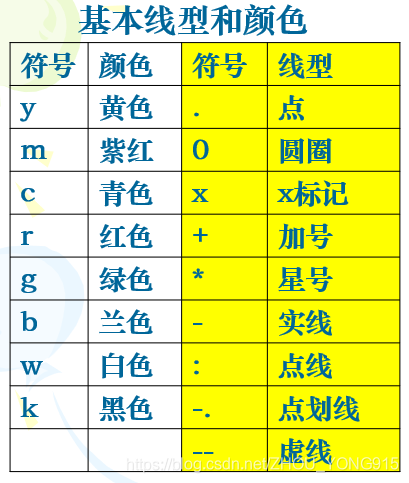
\includegraphics[width=0.9\linewidth]{graph_sign.png}
    \caption{系统响应曲线对比}
    \end{figure}

\section{结论}
仿真结果表明...（结论内容）...


    @inproceedings
    {key,
    author    = {作者},
    title     = {论文标题},
    booktitle = {会议名称},
    year      = {年份},
    pages     = {页码},
    address   = {会议地点}
    }



\end{document}